\section{Apriori\-Reverse$<$ Sets\-Type, Measure, Word, Cand\_\-Data\-Struct $>$ Class Template Reference}
\label{class_apriori_reverse}\index{AprioriReverse@{AprioriReverse}}
Functor finding the theory and/or the negative border and/or the positive border using the {\bf Apriori}{\rm (p.\,\pageref{class_apriori})} strategy but with a top down exploration of the search space.  


{\tt \#include $<$Apriori\-Reverse.hxx$>$}

Inheritance diagram for Apriori\-Reverse$<$ Sets\-Type, Measure, Word, Cand\_\-Data\-Struct $>$::\begin{figure}[H]
\begin{center}
\leavevmode
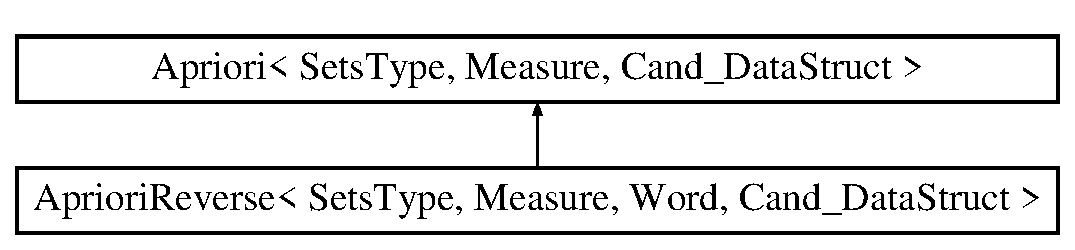
\includegraphics[height=2cm]{class_apriori_reverse}
\end{center}
\end{figure}
\subsection*{Public Member Functions}
\begin{CompactItemize}
\item 
{\bf Apriori\-Reverse} ()\label{class_apriori_reverse_18dd0f31ac2d8bc6d9036be8104bb6b8}

\begin{CompactList}\small\item\em Constructor. \item\end{CompactList}\item 
template$<$class Init\-Functor, class Predicate, class Output\-Theory, class Output\-Bd\-P, class Output\-Bd\-N, class f$>$ void {\bf operator()} (Init\-Functor \&init, {\bf Predicate} \&pred, Output\-Theory $\ast$theory, Output\-Bd\-P $\ast$bd\-P, Output\-Bd\-N $\ast$bd\-N, f \&word\-To\-Set)
\begin{CompactList}\small\item\em Functor operator that executes the algorithm. \item\end{CompactList}\item 
template$<$class Init\-Functor, class Predicate, class Output\-Theory, class Output\-Bd\-P, class Output\-Bd\-N$>$ void {\bf operator()} (Init\-Functor \&init, {\bf Predicate} \&pred, Output\-Theory $\ast$theory, Output\-Bd\-P $\ast$bd\-P, Output\-Bd\-N $\ast$bd\-N)
\begin{CompactList}\small\item\em Functor operator that executes the algorithm. \item\end{CompactList}\item 
template$<$class Init\-Functor, class Predicate, class Output\-Theory, class Output\-Bd\-P, class Output\-Bd\-N, class f, class Stop\-Iteration$>$ void {\bf operator()} (Init\-Functor \&init, {\bf Predicate} \&pred, Output\-Theory $\ast$theory, Output\-Bd\-P $\ast$bd\-P, Output\-Bd\-N $\ast$bd\-N, Stop\-Iteration $\ast$stop\-Ite, f \&word\-To\-Set)
\begin{CompactList}\small\item\em Functor operator that executes the algorithm and stop his execution when the functor passed in parameter return false. \item\end{CompactList}\item 
template$<$class Init\-Functor, class Predicate, class Output\-Theory, class Output\-Bd\-P, class Output\-Bd\-N, class Stop\-Iteration$>$ void {\bf operator()} (Init\-Functor \&init, {\bf Predicate} \&pred, Output\-Theory $\ast$theory, Output\-Bd\-P $\ast$bd\-P, Output\-Bd\-N $\ast$bd\-N, Stop\-Iteration $\ast$stop\-Ite)
\begin{CompactList}\small\item\em Functor operator that executes the algorithm and stop his execution when the functor passed in parameter return false. \item\end{CompactList}\end{CompactItemize}


\subsection{Detailed Description}
\subsubsection*{template$<$class Sets\-Type = int, class Measure = Boolean, class Word = vector$<$ Sets\-Type $>$, class Cand\_\-Data\-Struct = PTree$<$Sets\-Type,Measure$>$$>$ class Apriori\-Reverse$<$ Sets\-Type, Measure, Word, Cand\_\-Data\-Struct $>$}

Functor finding the theory and/or the negative border and/or the positive border using the {\bf Apriori}{\rm (p.\,\pageref{class_apriori})} strategy but with a top down exploration of the search space. 

Moreover this class enables to stop the execution of the algorithm at an iteration wrt to a user defined functor. The template parameter Sets\-Type represents the type of the sets representing the elements of the language. The template parameter Measure is the type of the value eventually associated with the word of the language. The template parameter Cand\_\-Data\-Struct is the data structure type used to store the candidates generated by the algorithms. The template parameter Word represents the type of the elements of the language. 



\subsection{Member Function Documentation}
\index{AprioriReverse@{Apriori\-Reverse}!operator()@{operator()}}
\index{operator()@{operator()}!AprioriReverse@{Apriori\-Reverse}}
\subsubsection{\setlength{\rightskip}{0pt plus 5cm}template$<$class Sets\-Type = int, class Measure = Boolean, class Word = vector$<$ Sets\-Type $>$, class Cand\_\-Data\-Struct = PTree$<$Sets\-Type,Measure$>$$>$ template$<$class Init\-Functor, class Predicate, class Output\-Theory, class Output\-Bd\-P, class Output\-Bd\-N, class Stop\-Iteration$>$ void {\bf Apriori\-Reverse}$<$ Sets\-Type, Measure, Word, Cand\_\-Data\-Struct $>$::operator() (Init\-Functor \& {\em init}, {\bf Predicate} \& {\em pred}, Output\-Theory $\ast$ {\em theory}, Output\-Bd\-P $\ast$ {\em bd\-P}, Output\-Bd\-N $\ast$ {\em bd\-N}, Stop\-Iteration $\ast$ {\em stop\-Ite})\hspace{0.3cm}{\tt  [inline]}}\label{class_apriori_reverse_a8018f226acaaa0047cf1386ed189e08}


Functor operator that executes the algorithm and stop his execution when the functor passed in parameter return false. 

\begin{Desc}
\item[Parameters:]
\begin{description}
\item[{\em init}]functor initializing the interesting items wrt predicate. \item[{\em pred}]the predicate \item[{\em theory}]output the theory in the given objet (must have a push\_\-back( container, measure ) method). \item[{\em bd\-P}]output the positive border in the given objet (must have a push\_\-back( container, measure ) method). \item[{\em bd\-N}]output the negative border in the given objet (must have a push\_\-back( container, measure ) method). \item[{\em stop\-Ite}]functor stop that stop the execution of the algorithm before the end. \item[{\em word\-To\-Set}]transform words of the language studied in sets. \end{description}
\end{Desc}


Reimplemented from {\bf Apriori$<$ Sets\-Type, Measure, Cand\_\-Data\-Struct $>$} {\rm (p.\,\pageref{class_apriori_117edc08779546395973171927fb8a77})}.\index{AprioriReverse@{Apriori\-Reverse}!operator()@{operator()}}
\index{operator()@{operator()}!AprioriReverse@{Apriori\-Reverse}}
\subsubsection{\setlength{\rightskip}{0pt plus 5cm}template$<$class Sets\-Type = int, class Measure = Boolean, class Word = vector$<$ Sets\-Type $>$, class Cand\_\-Data\-Struct = PTree$<$Sets\-Type,Measure$>$$>$ template$<$class Init\-Functor, class Predicate, class Output\-Theory, class Output\-Bd\-P, class Output\-Bd\-N, class f, class Stop\-Iteration$>$ void {\bf Apriori\-Reverse}$<$ Sets\-Type, Measure, Word, Cand\_\-Data\-Struct $>$::operator() (Init\-Functor \& {\em init}, {\bf Predicate} \& {\em pred}, Output\-Theory $\ast$ {\em theory}, Output\-Bd\-P $\ast$ {\em bd\-P}, Output\-Bd\-N $\ast$ {\em bd\-N}, Stop\-Iteration $\ast$ {\em stop\-Ite}, f \& {\em word\-To\-Set})\hspace{0.3cm}{\tt  [inline]}}\label{class_apriori_reverse_d898f211e89442230c64651031388e3d}


Functor operator that executes the algorithm and stop his execution when the functor passed in parameter return false. 

\begin{Desc}
\item[Parameters:]
\begin{description}
\item[{\em init}]functor initializing the interesting items wrt predicate. \item[{\em pred}]the predicate \item[{\em theory}]output the theory in the given objet (must have a push\_\-back( container, measure ) method). \item[{\em bd\-P}]output the positive border in the given objet (must have a push\_\-back( container, measure ) method). \item[{\em bd\-N}]output the negative border in the given objet (must have a push\_\-back( container, measure ) method). \item[{\em stop\-Ite}]functor stop that stop the execution of the algorithm before the end. \item[{\em word\-To\-Set}]transform words of the language studied in sets. \end{description}
\end{Desc}


Reimplemented from {\bf Apriori$<$ Sets\-Type, Measure, Cand\_\-Data\-Struct $>$} {\rm (p.\,\pageref{class_apriori_4ccc3fe5ae7ecaa9efffcdc41d1888ed})}.\index{AprioriReverse@{Apriori\-Reverse}!operator()@{operator()}}
\index{operator()@{operator()}!AprioriReverse@{Apriori\-Reverse}}
\subsubsection{\setlength{\rightskip}{0pt plus 5cm}template$<$class Sets\-Type = int, class Measure = Boolean, class Word = vector$<$ Sets\-Type $>$, class Cand\_\-Data\-Struct = PTree$<$Sets\-Type,Measure$>$$>$ template$<$class Init\-Functor, class Predicate, class Output\-Theory, class Output\-Bd\-P, class Output\-Bd\-N$>$ void {\bf Apriori\-Reverse}$<$ Sets\-Type, Measure, Word, Cand\_\-Data\-Struct $>$::operator() (Init\-Functor \& {\em init}, {\bf Predicate} \& {\em pred}, Output\-Theory $\ast$ {\em theory}, Output\-Bd\-P $\ast$ {\em bd\-P}, Output\-Bd\-N $\ast$ {\em bd\-N})\hspace{0.3cm}{\tt  [inline]}}\label{class_apriori_reverse_5266cde8d5a9455c9f9281e435754ca9}


Functor operator that executes the algorithm. 

\begin{Desc}
\item[Parameters:]
\begin{description}
\item[{\em init}]functor initializing the interesting items wrt predicate. \item[{\em pred}]the predicate \item[{\em theory}]output the theory in the given objet (must have a push\_\-back( container, measure ) method). \item[{\em bd\-P}]output the positive border in the given objet (must have a push\_\-back( container, measure ) method). \item[{\em bd\-N}]output the negative border in the given objet (must have a push\_\-back( container, measure ) method). \end{description}
\end{Desc}


Reimplemented from {\bf Apriori$<$ Sets\-Type, Measure, Cand\_\-Data\-Struct $>$} {\rm (p.\,\pageref{class_apriori_f0a2087314d1753cc3dd397c4a3f3dda})}.\index{AprioriReverse@{Apriori\-Reverse}!operator()@{operator()}}
\index{operator()@{operator()}!AprioriReverse@{Apriori\-Reverse}}
\subsubsection{\setlength{\rightskip}{0pt plus 5cm}template$<$class Sets\-Type = int, class Measure = Boolean, class Word = vector$<$ Sets\-Type $>$, class Cand\_\-Data\-Struct = PTree$<$Sets\-Type,Measure$>$$>$ template$<$class Init\-Functor, class Predicate, class Output\-Theory, class Output\-Bd\-P, class Output\-Bd\-N, class f$>$ void {\bf Apriori\-Reverse}$<$ Sets\-Type, Measure, Word, Cand\_\-Data\-Struct $>$::operator() (Init\-Functor \& {\em init}, {\bf Predicate} \& {\em pred}, Output\-Theory $\ast$ {\em theory}, Output\-Bd\-P $\ast$ {\em bd\-P}, Output\-Bd\-N $\ast$ {\em bd\-N}, f \& {\em word\-To\-Set})\hspace{0.3cm}{\tt  [inline]}}\label{class_apriori_reverse_f82618122967f0c6da9c4de5ea60a367}


Functor operator that executes the algorithm. 

\begin{Desc}
\item[Parameters:]
\begin{description}
\item[{\em init}]functor initializing the interesting items wrt predicate. \item[{\em pred}]the predicate \item[{\em theory}]output the theory in the given objet (must have a push\_\-back( container, measure ) method). \item[{\em bd\-P}]output the positive border in the given objet (must have a push\_\-back( container, measure ) method). \item[{\em bd\-N}]output the negative border in the given objet (must have a push\_\-back( container, measure ) method). \item[{\em word\-To\-Set}]transform words of the language studied in sets. \end{description}
\end{Desc}


Reimplemented from {\bf Apriori$<$ Sets\-Type, Measure, Cand\_\-Data\-Struct $>$} {\rm (p.\,\pageref{class_apriori_36d7a2cdad2a8c459f2b44e3ab460591})}.

The documentation for this class was generated from the following file:\begin{CompactItemize}
\item 
F:/i\-Zi/algorithms/Apriori\-Reverse.hxx\end{CompactItemize}
